\chapter{Quantised vortices in droplets}\label{sec:quant-vort}
	\lettrine[lines=4]{\color{activeColor}O}{ne} of the most unambiguous signatures of the quantum mechanical nature of a substance ---and indeed of superfluidity--- is the appearance of quantised vortices. The work in this part of the thesis is mostly inspired and motivated by experiments performed by Gomez, Loginov and Vilesov\citep{Gomez:2012,Gom14}.
	
	\section{Introduction}
		Normal fluids rotate rigidly when their containers are spinning at low angular velocities, with an angular velocity $v_\perp$ proportional to the distance $r$ from the axis of rotation $v_\perp\propto r$. This behaviour changes completely when the normal fluid is replaced by a superfluid like liquid helium below $T_\lambda$; below a critical angular velocity, the fluid remains at rest. When the angular velocity of the container is increased above this critical velocity, one or more quantised vortices are nucleated. In contrast to a normal fluid, the angular velocity $v_s$ of a superfluid directly outside the vortex core is inversely proportional to the distance from the vortex core $v_s\propto 1/r$. These vortices can be described by an effective wave function and a quantised circulation $\Gamma$ of the velocity field
		\begin{align}
			\Gamma=s\frac{h}{m}	
		\end{align}
		where $s$ is the angular momentum quantum number, $h$ is Planck’s constant and $m$ is the mass of the $^4$He atom (see \eq{eq:circulation} for a derivation and\rfs{Don91,Pit03}). An important aspect in the study of vorticity in finite systems is the energy and momentum transfer between vortices and surface excitations, because they determine nucleation dynamics, shape and the stability of vortices. But the study of quantum vortices is no longer confined to superfluids like liquid helium. Recently\citep{Pit03,Fetter2009} it has been extended to BECs confined in magnetic traps. Contrary to confined BECs, superfluid helium droplets are self-contained systems that do not require an external trap to keep them from falling apart. Moreover, they provide an opportunity to study the regime of a strongly interacting quantum system. The width of vortex cores, about 0.2~nm\citep{Don91} in superfluid helium-4, is small compared to the size of the droplets (typically a diameter of $\sim$4.4--10.9~nm), suggesting a rich variety of three-dimensional phenomena. Quantum vortices in superfluid droplets are therefore a very active field of interest\citep{Clo98,Lehmann2003,Bar06,Sti06}. 
		
		Recently, Gomez \emph{et al}. performed experiments\citep{Gomez:2012} where vortices inside superfluid $^4$He nanodroplets, produced by the expansion of liquid helium, were doped with Ag atoms which then clustered along the vortex lines in the droplets. The helium droplets needed by these kind of experiments need to be larger than the ones used before for single atom spectroscopy and dynamics studies, because they need to be big enough to be able to host an array of vortices, doped with many Ag clusters.
		
		A schematic of the experimental principle is shown in \fig{fig:vortex-machine}. Helium droplets are produced by expansion of He, at 20~bars and a temperature $T_0$=5.4--7~K, into a vacuum through a nozzle. The droplets cool down rapidly by evaporation and reach a temperature of 0.37~K\citep{Hartmann1995}. This temperature is well below the superfluid transition temperature $T_\lambda$=2.17~K\citep{Don91,Pit03}. Further along the apparatus, the droplets capture about 10$^3$–10$^6$~Ag atoms in an oven\citep{Log11d}. The droplets are then collided against a thin carbon film substrate at room temperature\citep{Log11d}. When the droplets hit the carbon film they evaporate while leaving behind on the surface the Ag filaments, which are subsequently imaged via a transmission electron microscope (TEM).
		
		The ubiquity of elongated filament-shaped deposits (see \fig{fig:silver-filament}) shows that vortices are present in droplets larger than about 300~nm (about 10$^9$ atoms) and that their lifetime exceeds a few milliseconds.
		
		\begin{figure}[t]
			\begin{center}
				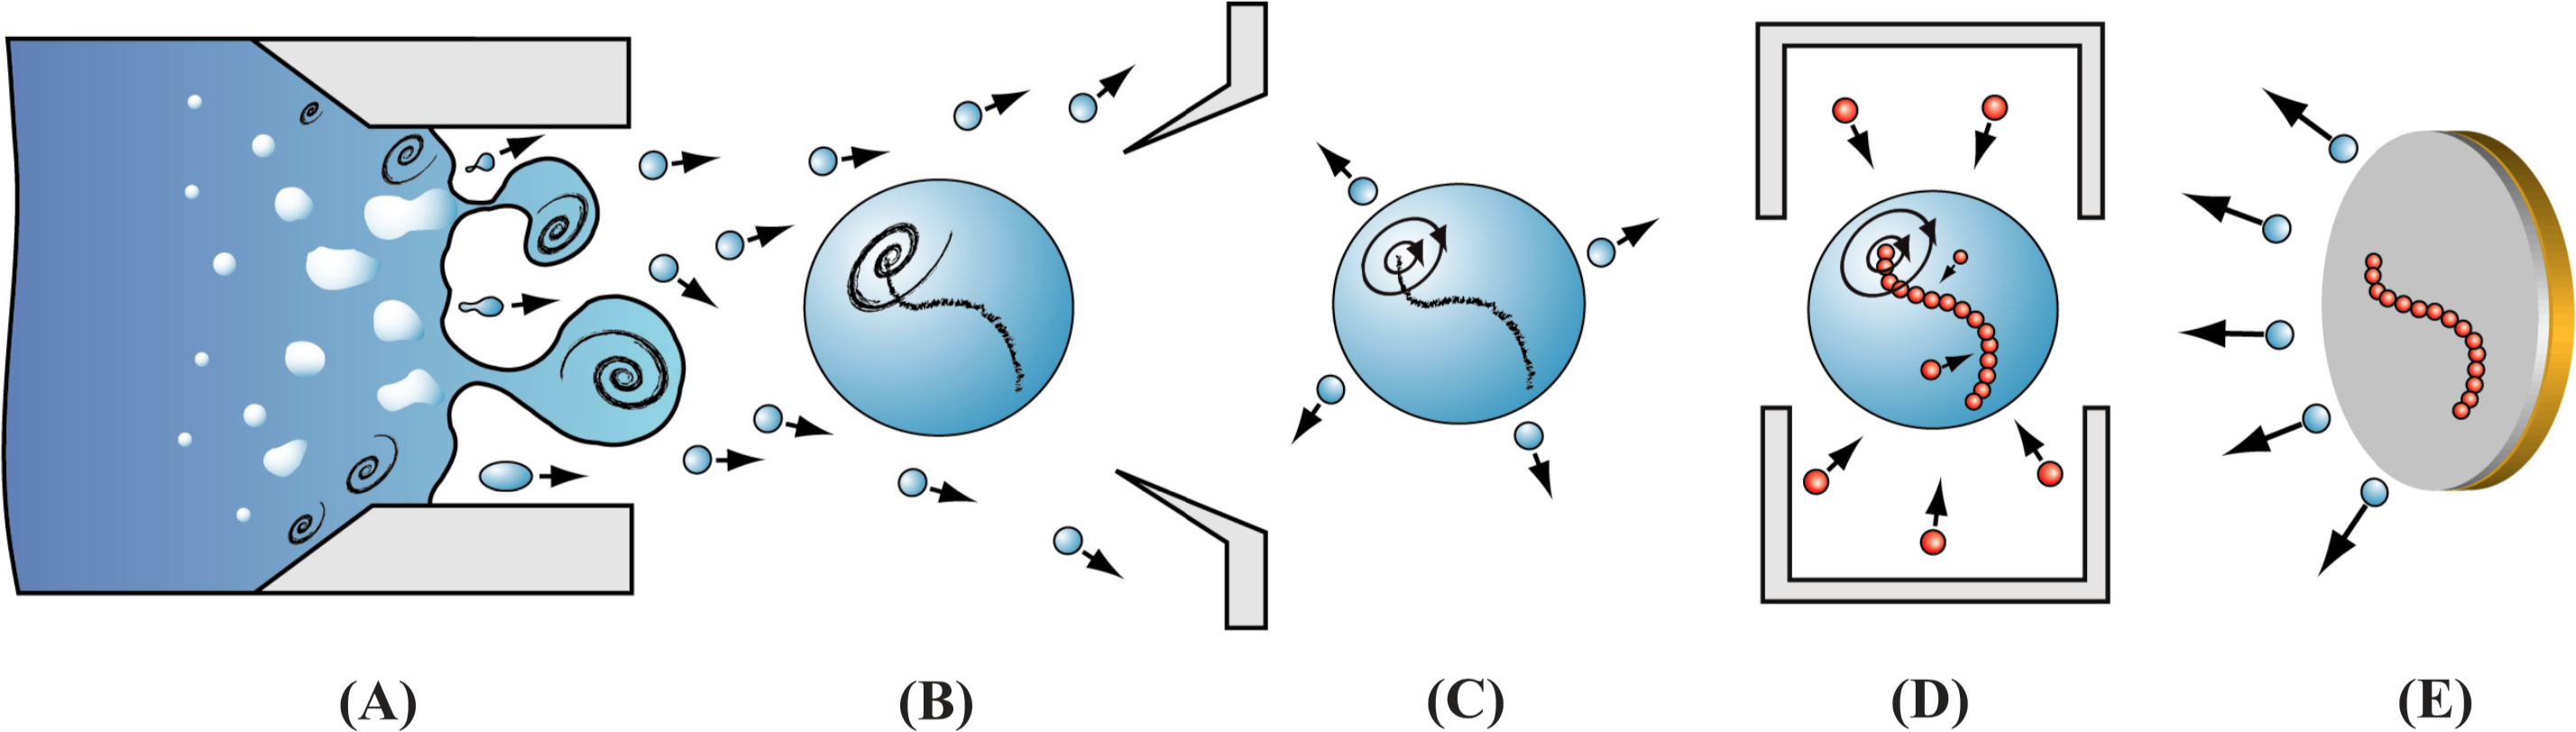
\includegraphics[width=\textwidth]{vortex-machine}
				\caption{Schematic of the experiment. (a) He fluid expands in vacuum and (b) breaks up into rotating droplets. (c) A quantum vortex is formed as a consequence of fast evaporative cooling of the droplet to below $T_\lambda$. (d) The droplet is doped with Ag atoms, which are attracted to the vortex core. (e) The droplet then collides with the carbon surface leaving behind the Ag trace, whereas the He evaporates. (Illustration courtesy of Gomez \emph{et al}. 2012, see\rf{Gomez:2012})}
				\label{fig:vortex-machine}
			\end{center}
		\end{figure}	
		
		Two years later Gomez \emph{et al}. reported\citep{Gom14} on the formation of quantum vortex lattices inside droplets. They used single-shot femtosecond X-ray coherent diffractive imaging to investigate the rotation of single, isolated superfluid helium-4 droplets containing about 10$^8$--10$^{11}$ atoms, corresponding to radii of $\simeq$100-1000~nm. The formation of quantum vortex lattices inside the droplets was confirmed by observing the characteristic Bragg patterns from xenon clusters trapped in the vortex cores (see \fig{fig:vortex-array}).
	
		\begin{figure}[t]
			\begin{center}
				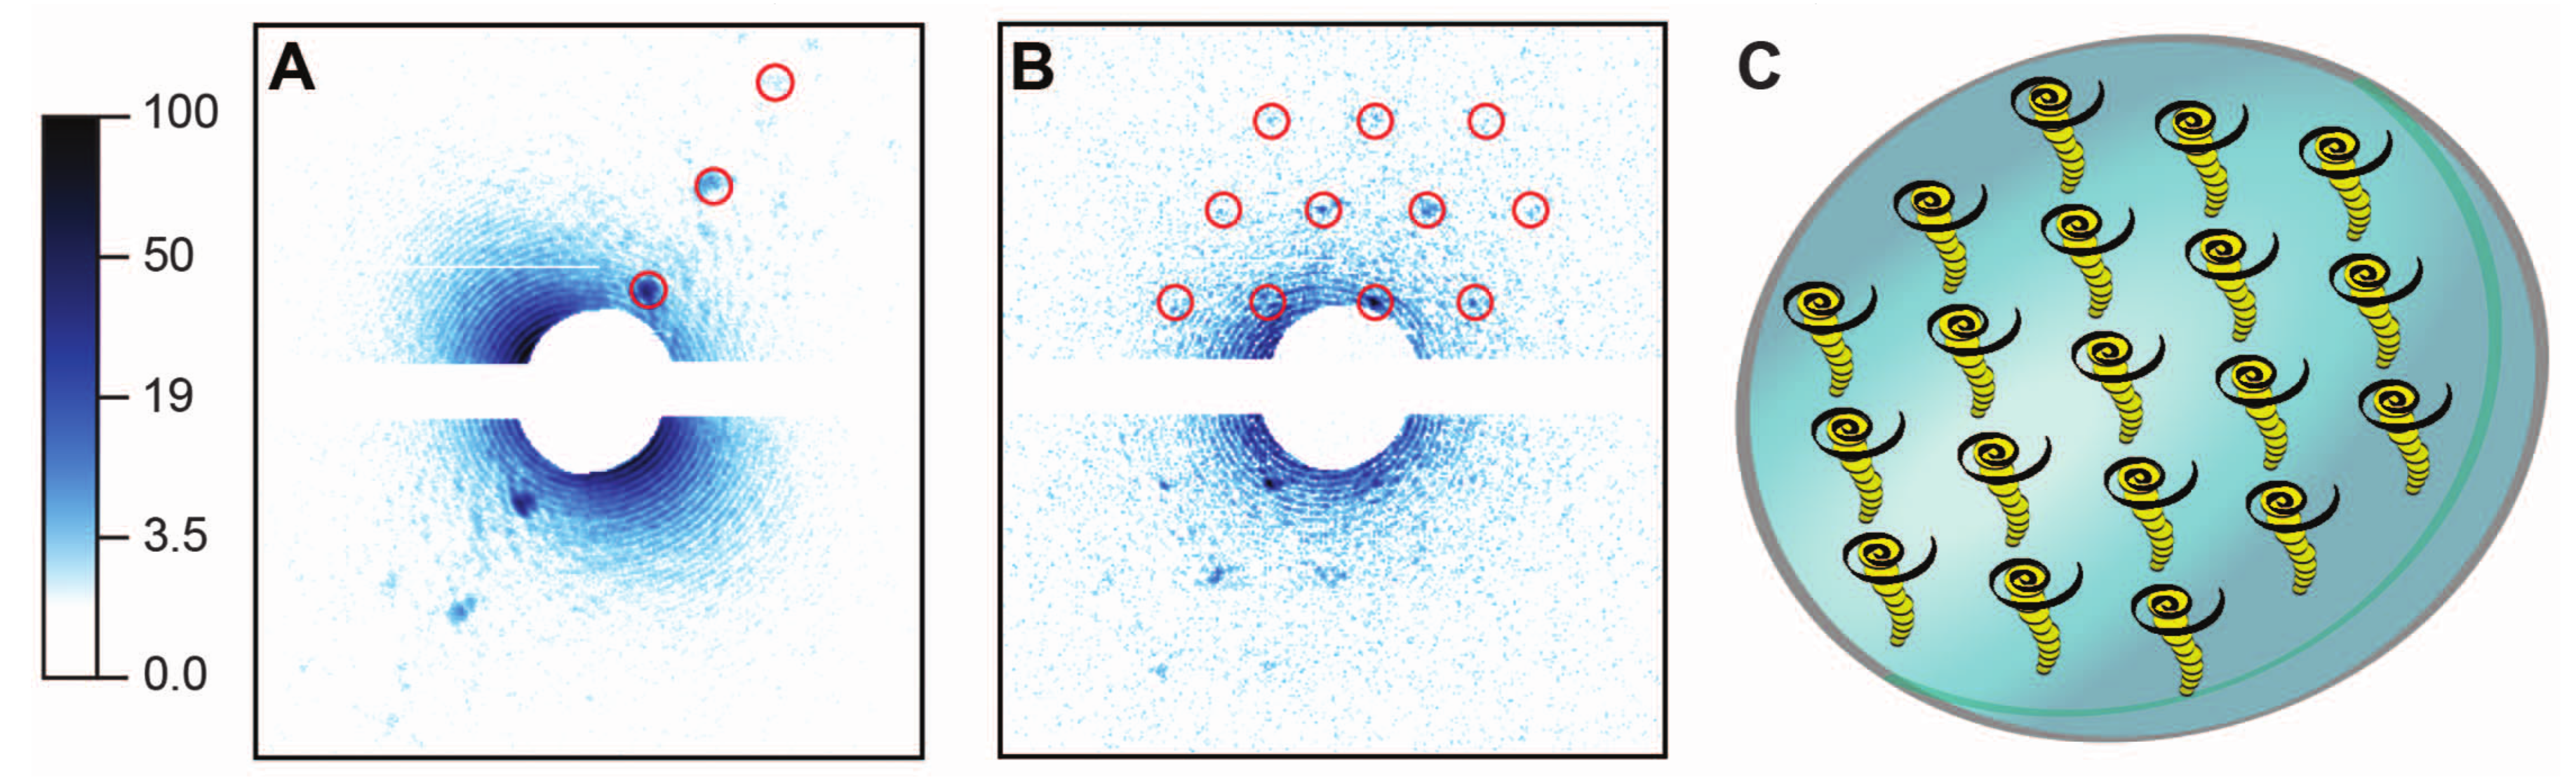
\includegraphics[width=\textwidth]{vortex-array}
				\caption{He droplets doped with Xe atoms. (A and B) X-ray diffraction images of doped droplets, displayed in a logarithmic intensity scale. (C) Droplet and embedded Xe clusters. Images in (A) and (B) correspond to tilted and parallel alignments of the vortex axes with respect to the incident x-ray beam, respectively. (Illustration courtesy of Gomez \emph{et al}. 2014, see\rf{Gom14})}
				\label{fig:vortex-array}
			\end{center}
		\end{figure}
		
	\section{Vortex arrays in $^4$He droplets doped with Ar atoms}
		The existence of ordered vortex lattices inside $^4$He droplets has been established  by the appearance of Bragg patterns from 
		Xe clusters trapped inside the vortex cores  in droplets made of $N= 10^8 - 10^{11}$ atoms
		(corresponding to radii from 100 to 1000 nm)\citep{Gom14,Jones2016}. We have 
		recently studied the stability of vortex 
		arrays made of up to $n_v=9$ vortices
		inside a $^4$He nanodroplet using the DFT approach\citep{Anc15}.  
		It was found that 
		the energetically favored structure for $n_v > 6$ is a ring 
		of vortices encircling a vortex at the center of the droplet.
		Fot $n_v=6$,  the 
		configuration with a six-vortex ring is found to have almost 
		the same energy as the five-fold ring
		plus a vortex at the center. The former structure 
		has been experimentally observed\citep{Gom14,Jones2016,Ber17}, 
		although classical vortex theory 
		predicts for it a much higher free energy cost than for the latter\citep{Cam79}.
		Similar equilibrium structures have been obtained within DFT for
		helium nanocylinders hosting vortex arrays\citep{Anc14}.
		
		\begin{figure}[!]
		\centerline{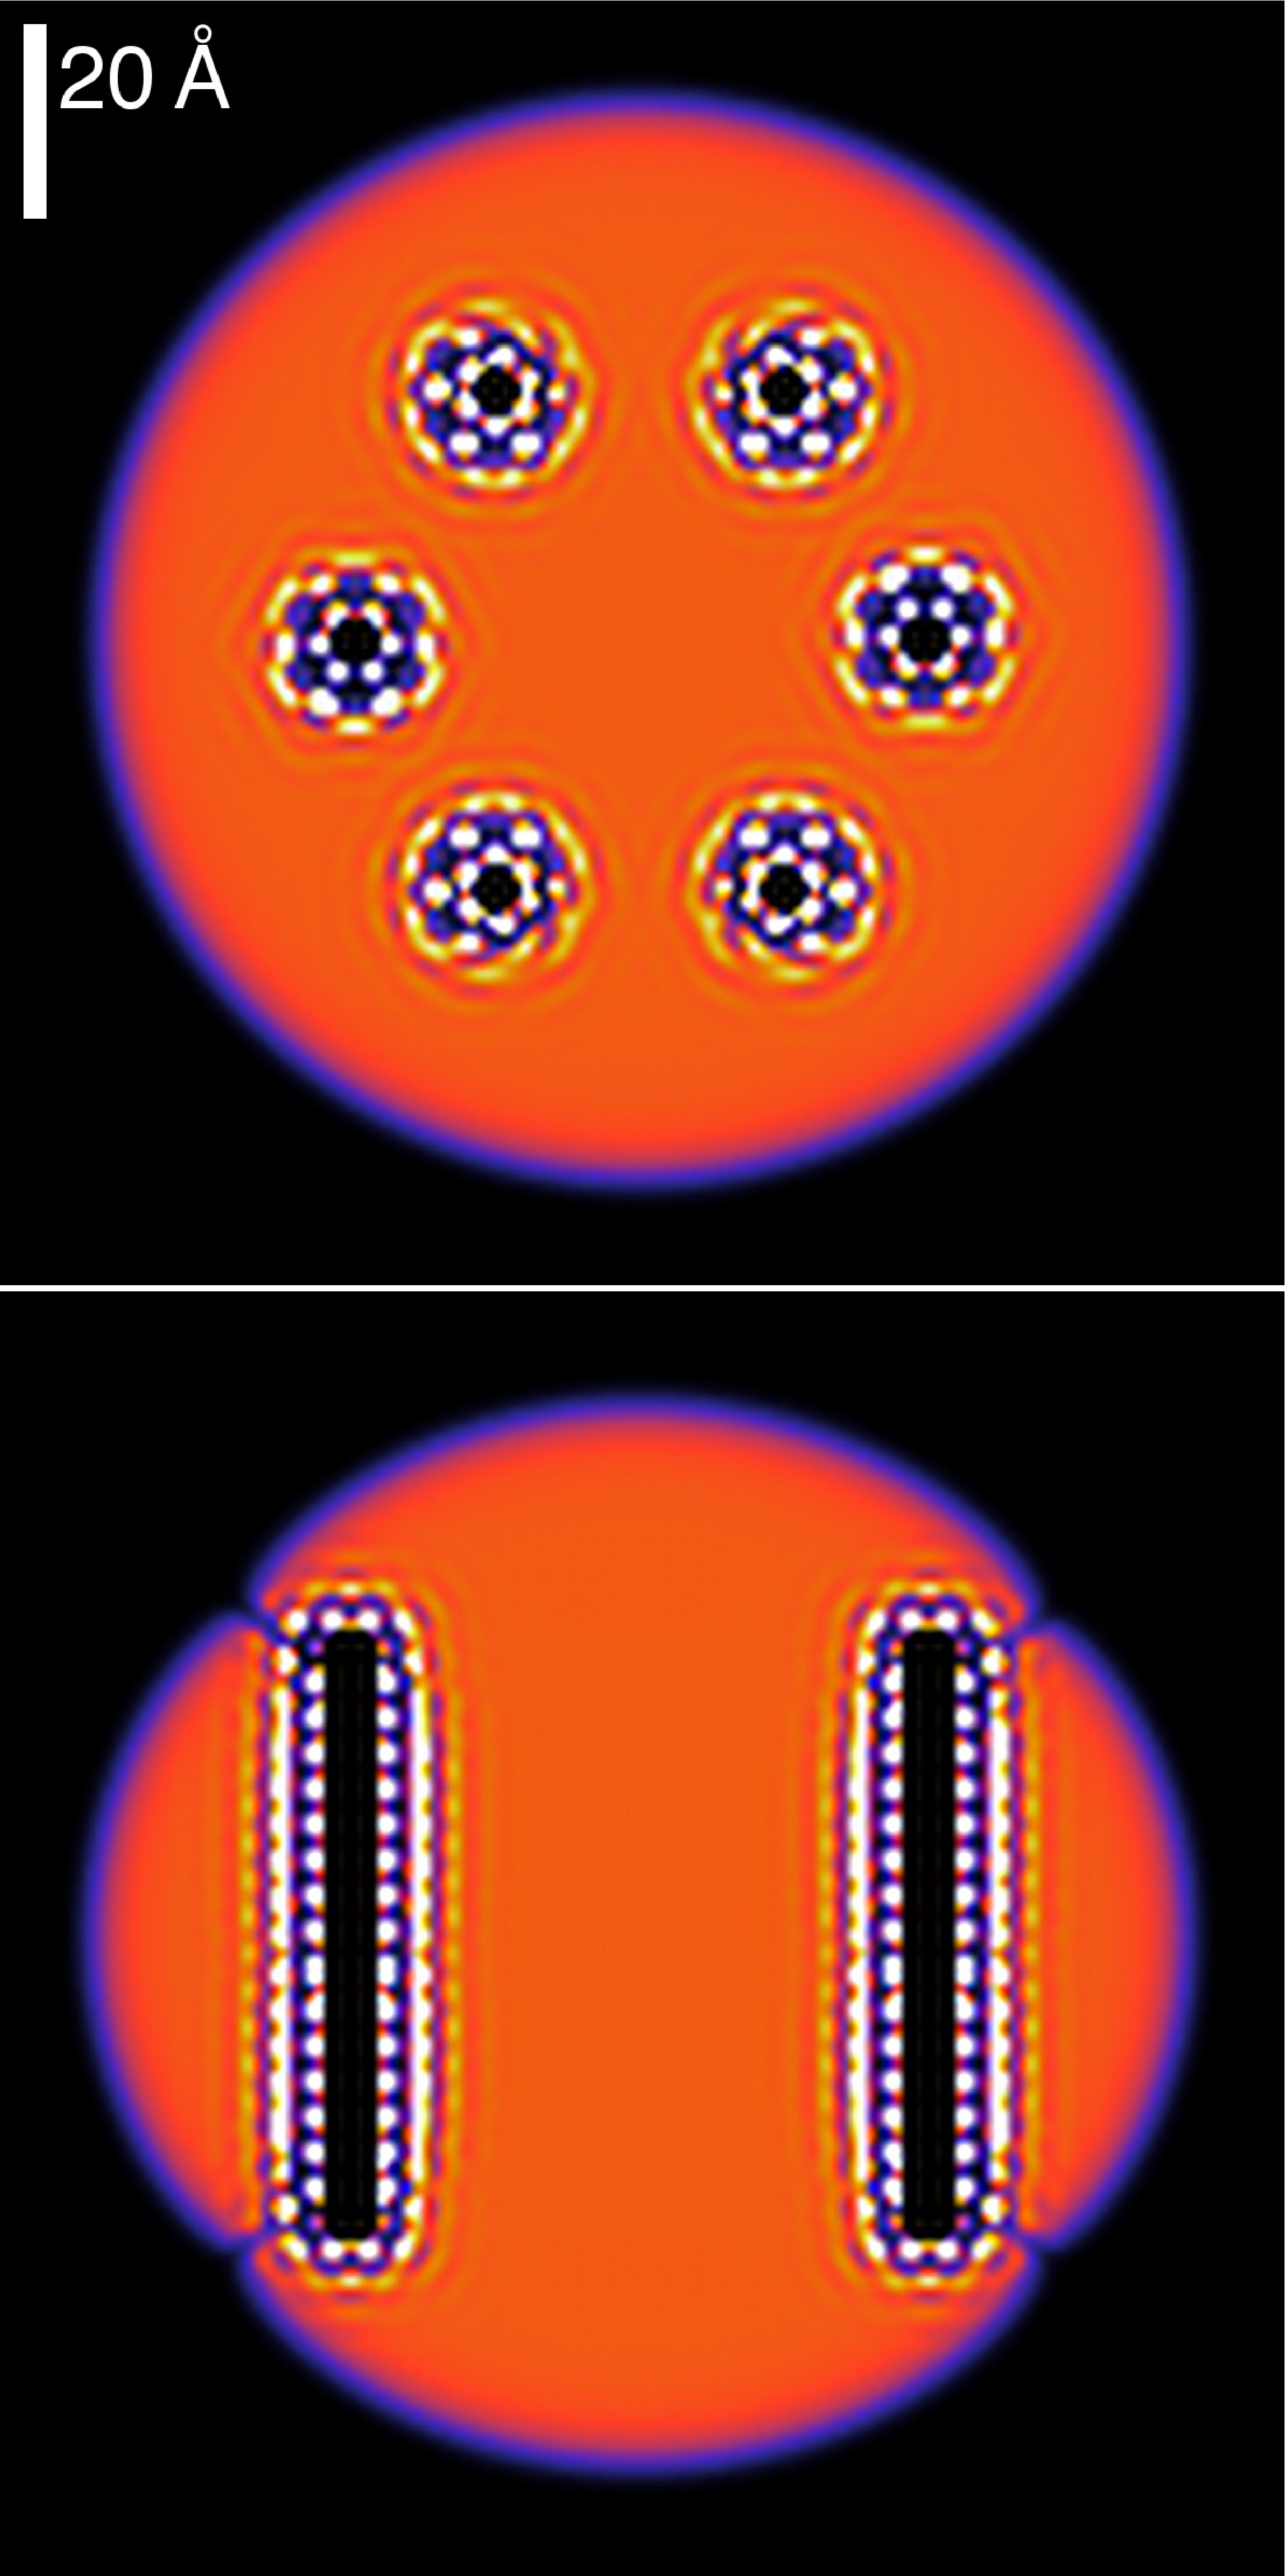
\includegraphics[width=0.6\linewidth,clip]{fig13}}
		\caption{\label{fig13-capture} 
		Helium droplet configuration hosting six vortices, each doped with a line of 
		regularly spaced Ar atoms (not represented). 
		The top figure shows the density in the $x-y$
		symmetry plane (top view), while the bottom figure shows a side view corresponding to the 
		$y-z$ plane. 
		As in some of the previous figures, the bright  spots are high density blobs appearing around the impurity atoms.
		}
		\end{figure}
		
		In the experiments of\rf{Jones2016} the diffraction images 
		show that rotating $^4$He nanodroplets of about 200 nm in diameter 
		contain a small number of symmetrically arranged quantum 
		vortices whose cores are filled with regularly spaced 
		Xe clusters. Unexpected large distances 
		of the vortices from the droplet center ($\sim$0.7--0.8 droplet radii) 
		are observed and explained as a result of the balance between 
		the contribution of the Xe atoms to the total angular momentum of the droplets and 
		the solvation potential of the embedded Xe atoms, which opposes the migration of vortices
		towards the droplet surface and their annihilation there, as it would
		happen instead in the case of undoped vortices for low values of the
		droplet rotational frequency.
		
		In practice, as more and more Xe atoms become
		attached to a vortex, they adopt the angular velocity of its
		revolution about the droplet center. 
		If the Xe capture is isotropic, the total angular momentum of the droplet is conserved, and 
		thus the angular momentum accompanying the Xe rotational motion must be
		transferred from the vortices to the impurities. This reduction in the angular momentum of the
		vortices causes them to move outwards, 
		resulting in the larger
		equilibrium distances of the vortices observed in 
		the experiments. The actual equilibrium radial positions
		result from a balance between this tendency to 
		move towards the droplet surface 
		and the solvation potential, 
		which tends instead to draw impurities towards the droplet
		center.
		
		We have looked for stationary configurations of a 6-vortex ring
		in a rotating He$_{15000}$ droplet by solving the
		EL equations in the corotating frame with a fixed
		angular velocity. Each vortex core is filled with Ar
		atoms, and the system is allowed to fully relax.
		In the end, the column of atoms inside each vortex core reaches an equilibrium structure 
		where the Ar atoms are separated by a distance which  is roughly that of the Ar dimer.
		One such configuration is shown in \fig{fig13-capture}. Note that 
		the vortex cores are almost straight lines, whereas in an
		undoped droplet rotating with the same velocity 
		the vortex lines would be bent, 
		as shown  e.g. in \fig{fig7-capture}.
		The Ar atoms are not shown in the Figure.
		The localized structures appearing in the vortex cores are 
		regions of highly inhomogeneous, high  $^4$He density
		resulting from the Ar-He attractive potential.
		% and \ref{fig9-capture}.
		
		The presence of impurities thus confers rigidity to the vortex lines,
		preventing them from bending. Yet, the small segment of the vortex line free from impurities bends so as to hit 
		the droplet surface perpendicularly, see the bottom \fig{fig13-capture}.
		Note that in the absence of vortices, Ar atoms initially placed
		in a linear chain structure would relax towards the lower energy, compact 
		configuration of an Ar cluster in the bulk of the droplet.
		However, once trapped by a vortex core, their collapse 
		into such a cluster structure does not occur,
		i.e. an energy barrier appears and prevents the formation of Ar
		clusters. 
		%As commented below, 
		Our simplified 
		description of the more complex experimental 
		conditions (where each vortex line hosts chains of regularly spaced
		atomic clusters, instead of chains of single atoms)
		is due to computational limitations.
		
		Our choice of Ar instead of Xe as a dopant is motivated by the weaker He-Ar and Ar-Ar interactions, which 
		facilitates the imaginary-time relaxation. The interaction of the helium environment with several close-by impurities increases the 
		strength of  dopant-droplet interaction, producing  
		helium localization around the impurities (snowball structures), see \fig{fig10-capture}. Stabilizing these
		structures is extremely time consuming, 
		especially when the He-impurity interaction is strong.
		Experiments were also carried out with Ar atoms as dopants, 
		but have not been analyzed yet.
		However, no significant difference is expected between argon and xenon, 
		neither from the experimental nor from the theoretical viewpoint.
		
		There are obvious differences in scales between our simulations and  
		 the actual experiments,  due to  computational 
		cost. In experiments heavier impurities are used (Xe), 
		the droplets are much larger
		and the doping is known to occur by filling the vortex cores with a chain 
		of equally spaced Xe clusters, each made of
		hundreds of atoms, instead of atom chains as done in our simulations.
		In spite of these differences, we find results which  
		qualitatively explain the unusual behavior of vortex lines 
		experimentally observed in doped rotating helium droplets.
		
		\begin{figure}[!]
		\centerline{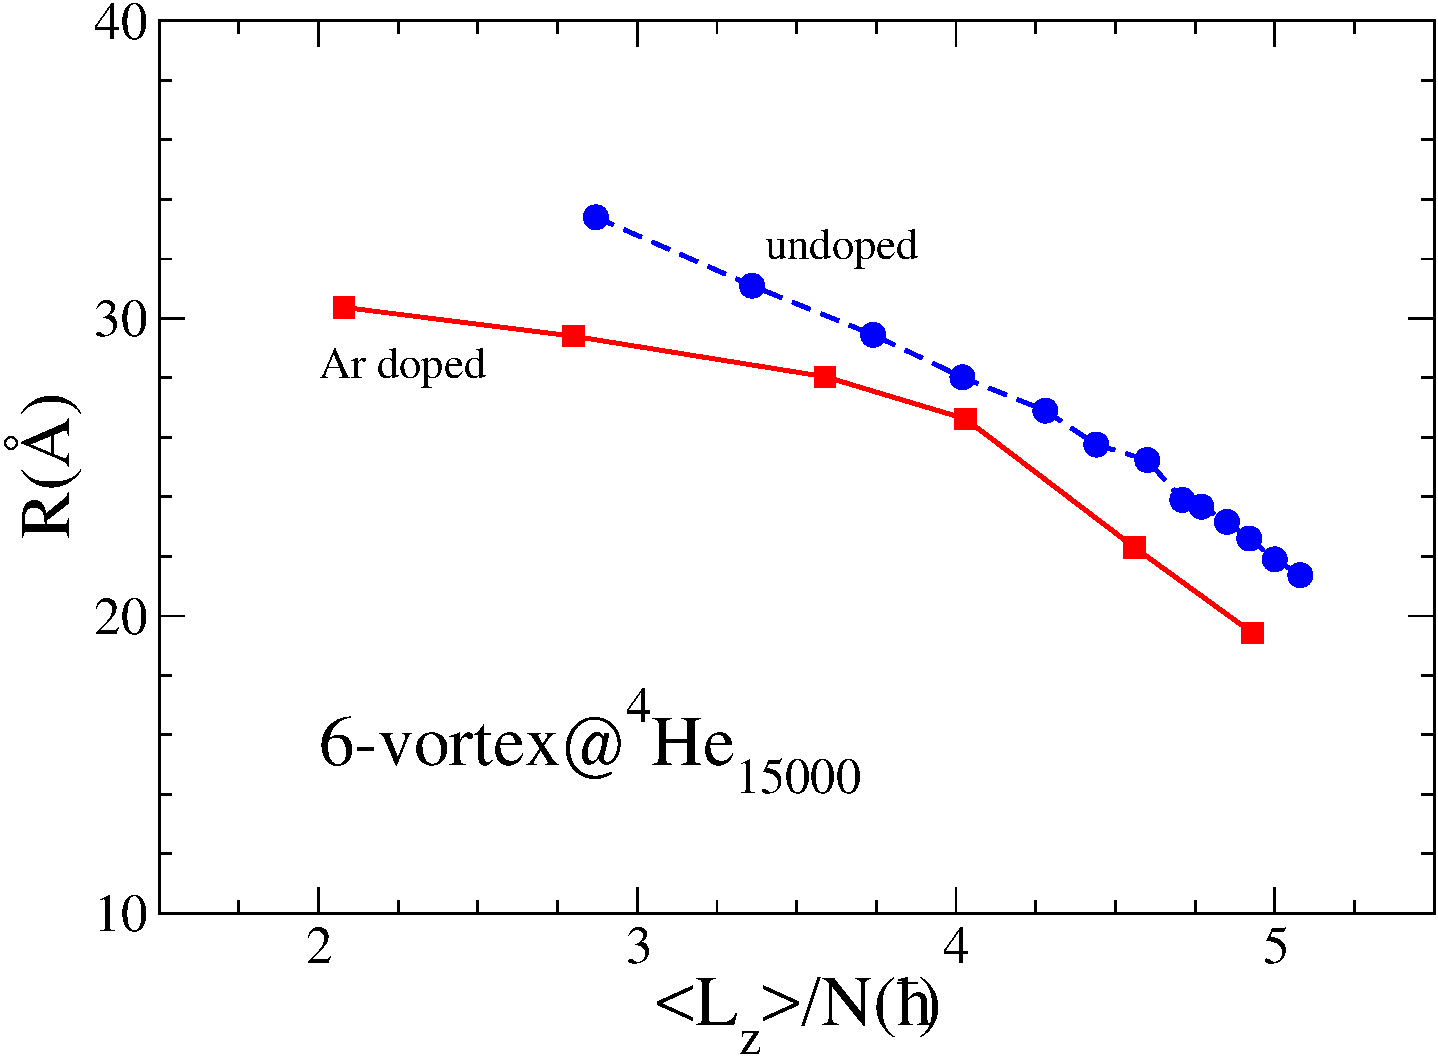
\includegraphics[width=0.9\linewidth,clip]{fig14}}
		\caption{\label{fig14-capture} 
		Calculated equilibrium distance of the 6-vortex ring
		from the droplet center as a function of the 
		angular momentum per He atom in units of $\hbar$. 
		The dots represent the results for undoped vortices, while the squares are the results for 
		Ar-doped vortices. The lines are drawn as a guide to the eye.
		}
		\end{figure}
		
		We have looked for the equilibrium structure of the Ar@6-vortex $^4$He$_{15000}$ droplet
		for different imposed values of the angular velocity
		of rotation. The results show that the doping inside each vortex core
		adds a substantial stability to the system, such that doped vortices are still 
		stable in a droplet rotating at rather low 
		values of the angular velocities, whereas undoped vortices
		for such values would be pushed towards the surface of the
		droplet and eventually expelled.
		The solvation potential effect becomes
		apparent below some critical 
		value of the angular velocity, where the vortices
		cease to move towards the surface and the 
		system reaches an equilibrium maximum distance
		of the vortices from the droplet center.
		This is shown in the \fig{fig14-capture}, 
		where we plot the radial distance of the vortices
		from the center as a function of the angular momentum
		of the system.
		Note how doped vortices are stable for values
		of the angular momentum well below the stability 
		limit of an undoped droplet.
		A similar behavior has been observed in the experiment (see for instance Figure 2 in the
		Supplemental Material of\rf{Jones2016}, see DOI:~\href{https://link.aps.org/doi/10.1103/PhysRevB.93.180510}{10.1103/PhysRevB.93.180510}).

\clearpage{\pagestyle{empty}\cleardoublepage}